\documentclass[tikz,border=8pt]{standalone}
\usepackage{amsmath}\usepackage{pgfplots}\pgfplotsset{compat=1.18}\usetikzlibrary{arrows.meta}
\definecolor{ink}{HTML}{334155}\definecolor{blue}{HTML}{6366F1}\definecolor{green}{HTML}{059669}\definecolor{orange}{HTML}{EA580C}
\begin{document}
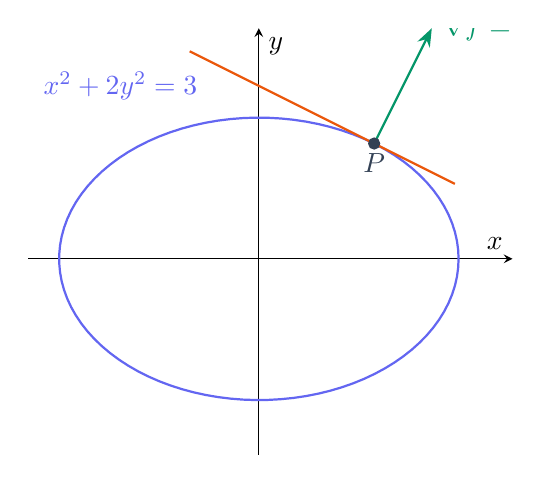
\begin{tikzpicture}[>=Stealth]\begin{axis}[width=11cm,height=7cm,axis equal image,axis lines=middle,xmin=-2,xmax=2.2,ymin=-1.7,ymax=2,xlabel=$x$,ylabel=$y$,ticks=none]
\addplot[blue,thick,domain=0:360,samples=100]({sqrt(3)*cos(x)},{sqrt(1.5)*sin(x)});
\addplot[green,thick,->]coordinates{(1,1)(1.5,2)}node[right]{$\nabla f=(2,4)$};
\addplot[orange,thick,domain=-.6:1.7]{1.5-.5*x};
\addplot[only marks,mark=*,ink]coordinates{(1,1)}node[below]{$P$};
\node[blue]at(axis cs:-1.2,1.5){$x^2+2y^2=3$};\end{axis}\end{tikzpicture}
\end{document}
